\chapter{Technologie cible et outils}\label{chap:met}
Le premier objectif proposé a été d'étudier le framework \kwplay et de s'assurer de la compatibilité de sa philosophie avec un projet de génération de code. Dans la section \ref{sec:pla} de ce chapitre, nous détaillerons les qualités de ce framework qui ont motivées la sélection de \kwplay pour ce projet. Dans un second temps (\cf{} section \ref{sec:pro}, nous aborderons le prototype que nous avons élaboré avec \kwplay. 


\section{Framework Play}\label{sec:pla}
\kwplay{} est un framework basé sur les langages Java et Scala permettant de la création d'applications web. De plus en plus de développeurs choisissent cet outil, qui est relativement récent, et qui présente de nombreux avantages. L'aspect \guim{prêt à l'emploi} (\textit{Plug'n Play}) permis par ses fonctionnalités par défaut le rendent efficace et rapide à mettre en place et à configurer. Le développement également est facilité, d'une part par par des mécanismes de compilation à la volée (\textit{shadow-build}) lors du chargement des pages, mais aussi par la mise à disposition de systèmes tests intégrées (JUnit, Selenium). Sa gestion des requêtes Web peut être bloquante ou non-bloquante (synchronisme). La génération des pages Web renvoyées peut être dynamisée grâce à un mécanismes de templating basé sur Scala. Enfin son architecture modulaire, composée de plugins et du \textit{design pattern} MVC (Modèle-Vue-Contrôleur), permettent une répartition claire du code source ce qui est propice à la démarche MDA. 


%TODO (terme à définir en début de rapport).

%{\huge $\Uparrow$ woua c'est nuull refractoring!!} Tu mens.



\section{Conception d’une maquette d’exemple}\label{sec:pro}

Nous nous sommes proposés de bâtir un mini-site Web basé sur \kwplay. L'ojectif est double :
\begin{itemize}
\item Nous familiariser avec le framework \kwplay et comprendre son fonctionnement.
\item Obtenir une maquette qui sera utilisée comme objectif de code à générer.
\end{itemize}

Le prototype que nous avons proposé est une implémentation simpliée d'un site marchand. Ce type de site web est en effet très courant, et il implique différents aspects et fonctionnalités : Stockage persistant de données (produits vendus), utilisation de formulaires (inscription des clients), utilisation de sessions (authentification des clients sur le site, et achats).

\begin{figure}[htb]
  \centering
  %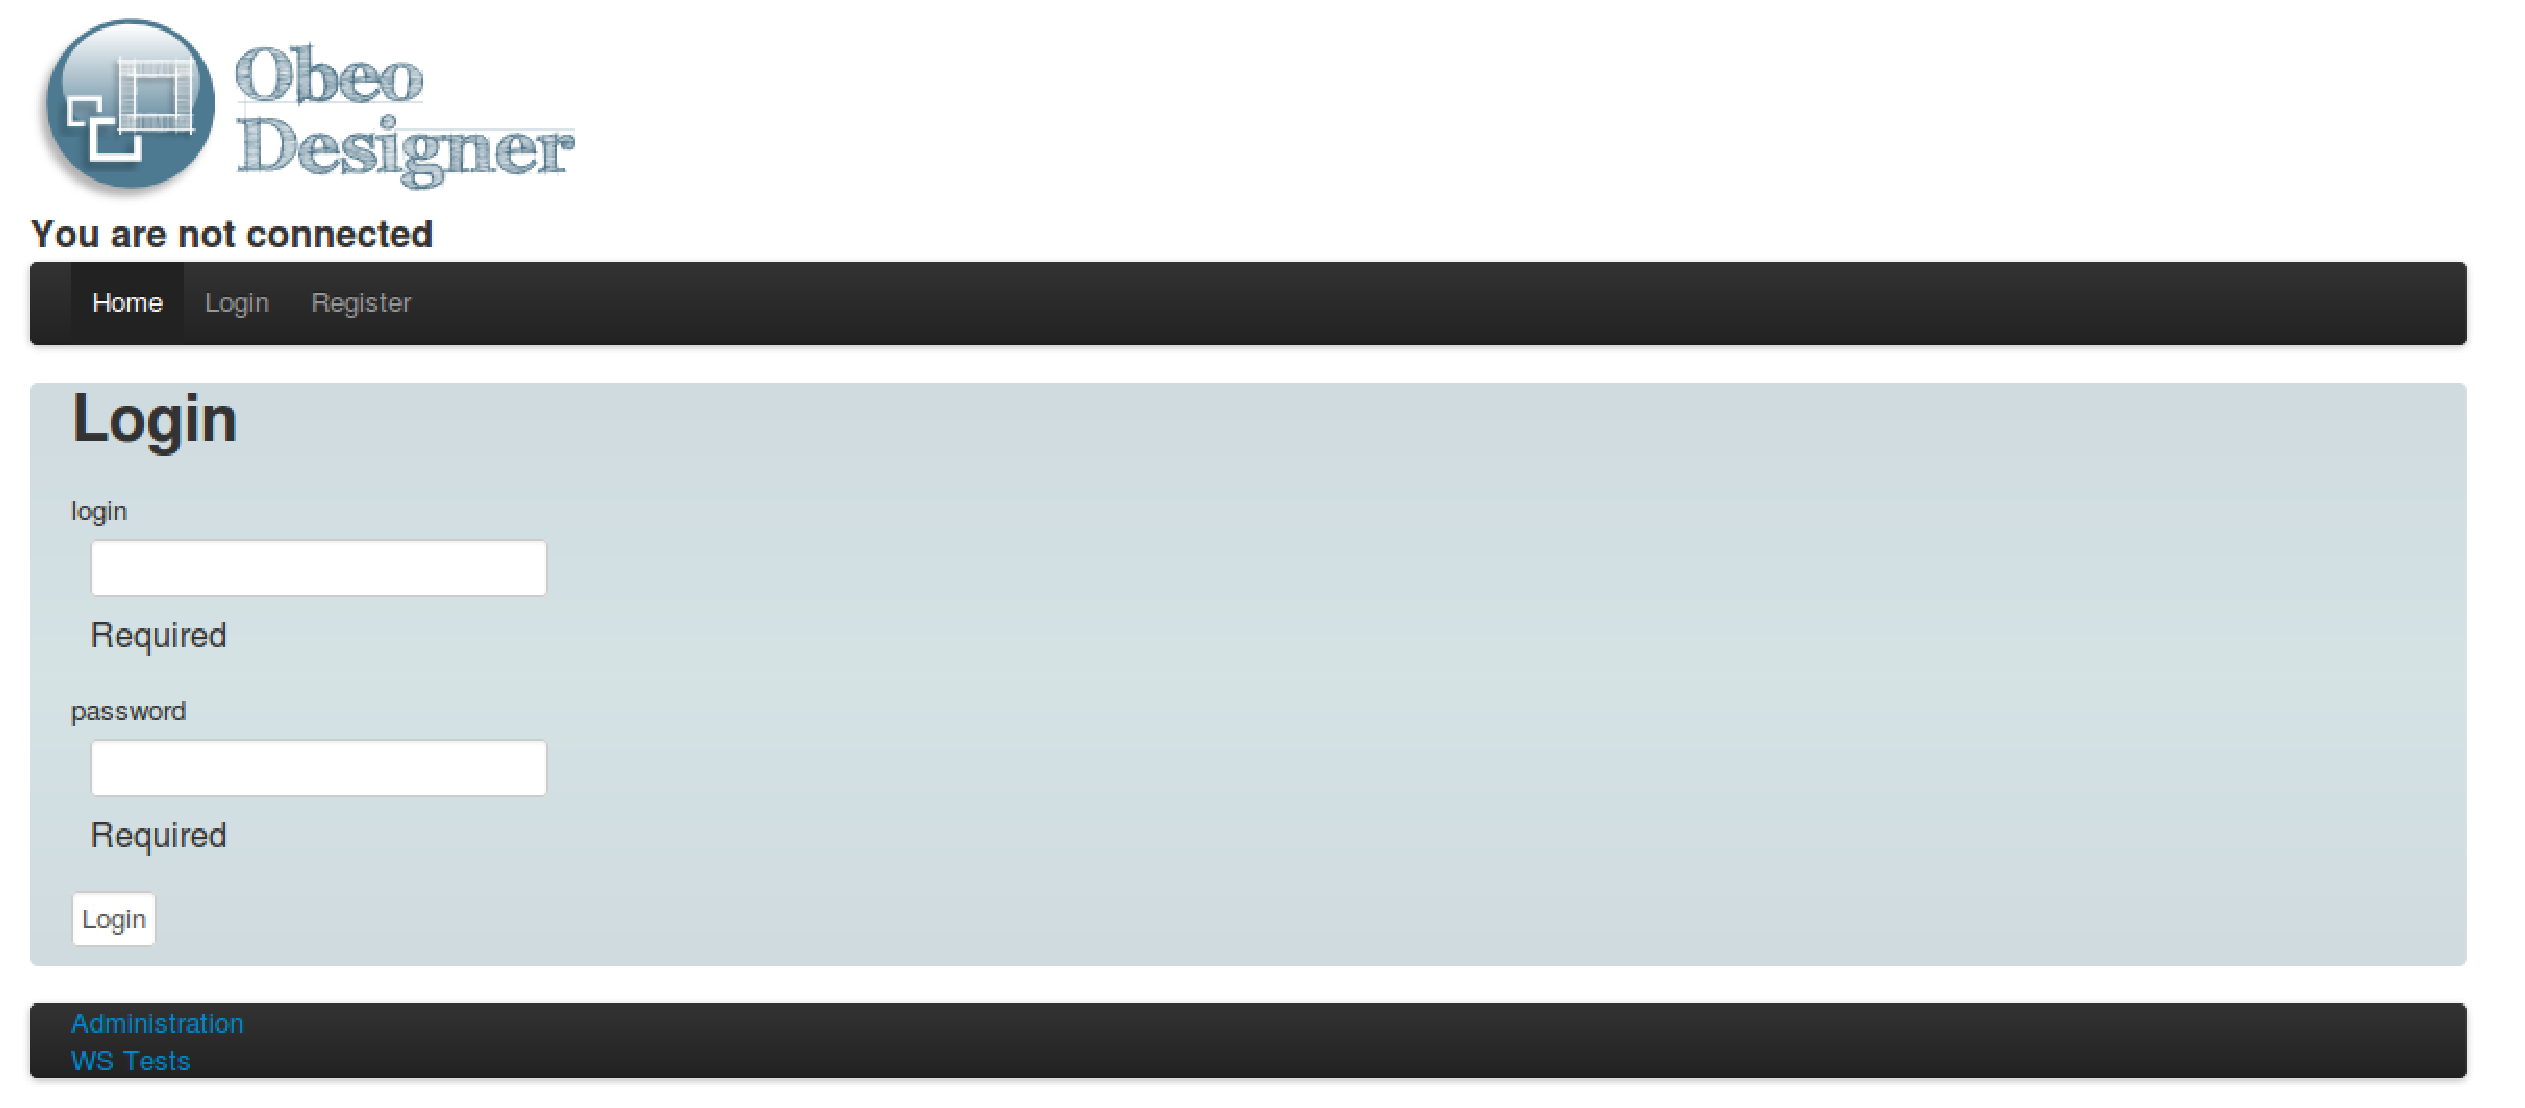
\includegraphics[scale=.2]{img/proto.eps}
  \caption{Prototype Play\_Shop}
  \label{fig:pro}
\end{figure}



%% \begin{figure}[htb]
%%   \centering
%%   \includegraphics[scale=.3]{img/Cin.eps}
%%   \caption{Méta model SOA}
%%   \label{fig:soa}
%% \end{figure}


%%  LocalWords:  framework play Scala web Plug'n shadow-build JUnit
%%  LocalWords:  Selenium non-bloquantes plugins MVC MDA woua nuull
%%  LocalWords:  refractoring implémentation Shop models Model Entity
%%  LocalWords:  méta-modèle model SOA blah bklah fdslmk
